\section{Introduction}
\label{sec:intro}

Ask a language model ``What country is An\'{i}bal Ponce a citizen of?'' and, a few dozen layers later, it answers ``Argentina''. On the way, the model's internal state at the last position of the prompt, from which the answer is produced, changes at every layer. This paper asks what shape that change has. Does the state wander, drift slowly toward the answer, or arrive somewhere definite? And if it arrives somewhere, is it the same somewhere for every question with the same answer?

It is. As a question passes through the network, its state moves into a region that it shares with every other question to which the model gives the same answer. Figure~\ref{fig:hero} shows this in Llama-3.1-8B. Early in the network, questions whose answers are twelve different countries form one tangled cloud. Within a few layers, most of them separate into one strand per country.

To study this, we built \NFacts{} factual questions from Wikidata whose answers recur: 62 countries, cities, languages and sports, each the answer to many questions. We asked them of four open models and recorded the state at every layer. For each answer and layer, we computed the \emph{answer centroid}: the average state of the questions to which the model gave that answer. We then measured, layer by layer, how often a question's state lies nearest its own answer's centroid, tested what the centroids encode, and moved states between centroids to see whether the model uses them. We find four things.

\emph{The answer becomes readable in a single layer} (Section~\ref{sec:step}). In each model, the share of questions whose state lies nearest its own answer's centroid jumps within one layer, at a depth that differs between models.

\emph{Centroids follow the model's answer, not the question} (Section~\ref{sec:shared}). The centroid of a country learned from questions about people also identifies that country in questions about towns and films. It survives rewording, and it is not simply the output direction of the answer word. When two models disagree, each state follows its own model's answer.

\emph{The model uses the centroids} (Section~\ref{sec:steer}). Moving a state to an answer's centroid after the jump makes the model give that answer. Random moves of the same size rarely do. Moves made before the jump have no effect, even when scaled up to the size of late moves.

\emph{Centroids reveal near misses} (Section~\ref{sec:errors}). Some wrong answers are near misses: shown the options, the model picks the right one. In a near miss, the right answer's centroid is among the nearest to the state. This tells near misses apart from real gaps in knowledge better than the model's confidence does.

\begin{figure*}[t]
\centering
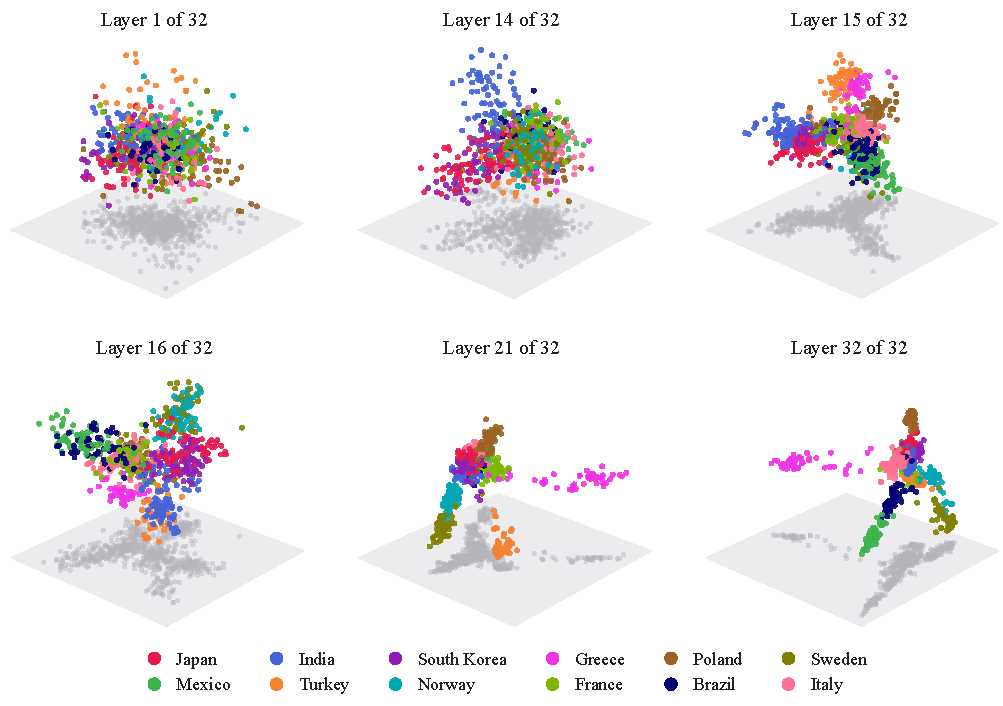
\includegraphics[width=\textwidth]{fig_hero.pdf}
\caption{\textbf{States of questions at six layers of Llama-3.1-8B.} Each point is one test question about a person, town or film whose answer is one of the twelve countries the model gave most often; colour is the country the model answered. Each panel shows the questions' states at one layer, projected onto the three directions that best separate the twelve countries among the training questions at that layer (found by linear discriminant analysis, LDA). At layer 1 all questions share one cloud, and at layer 14 a few countries, such as India, stand apart. At layer 15, where readability jumps (Section~\ref{sec:step}), most countries separate; by the last layer most form a strand of their own. Each panel is scaled separately; grey dots are shadows on the floor.}
\label{fig:hero}
\end{figure*}
